\documentclass{article}

% Language setting
% Replace `english' with e.g. `spanish' to change the document language
\usepackage[english]{babel}

% Set page size and margins
% Replace `letterpaper' with `a4paper' for UK/EU standard size
\usepackage[letterpaper,top=2cm,bottom=2cm,left=3cm,right=3cm,marginparwidth=1.75cm]{geometry}

% Useful packages
\usepackage{amsmath}
\usepackage{graphicx}
\usepackage{textalpha}
\usepackage{float}
\usepackage[colorlinks=true, allcolors=blue]{hyperref}

\title{Variable mechanical stiffness robotics arm testbed}
\author{Matthieu Prigent}

\begin{document}
\maketitle

\begin{abstract}
This document aims to summarize what was done in the development and building of testbed 2, and what was learned from it, for further development with testbed 3.
\end{abstract}

\begin{figure}[H]
\centering
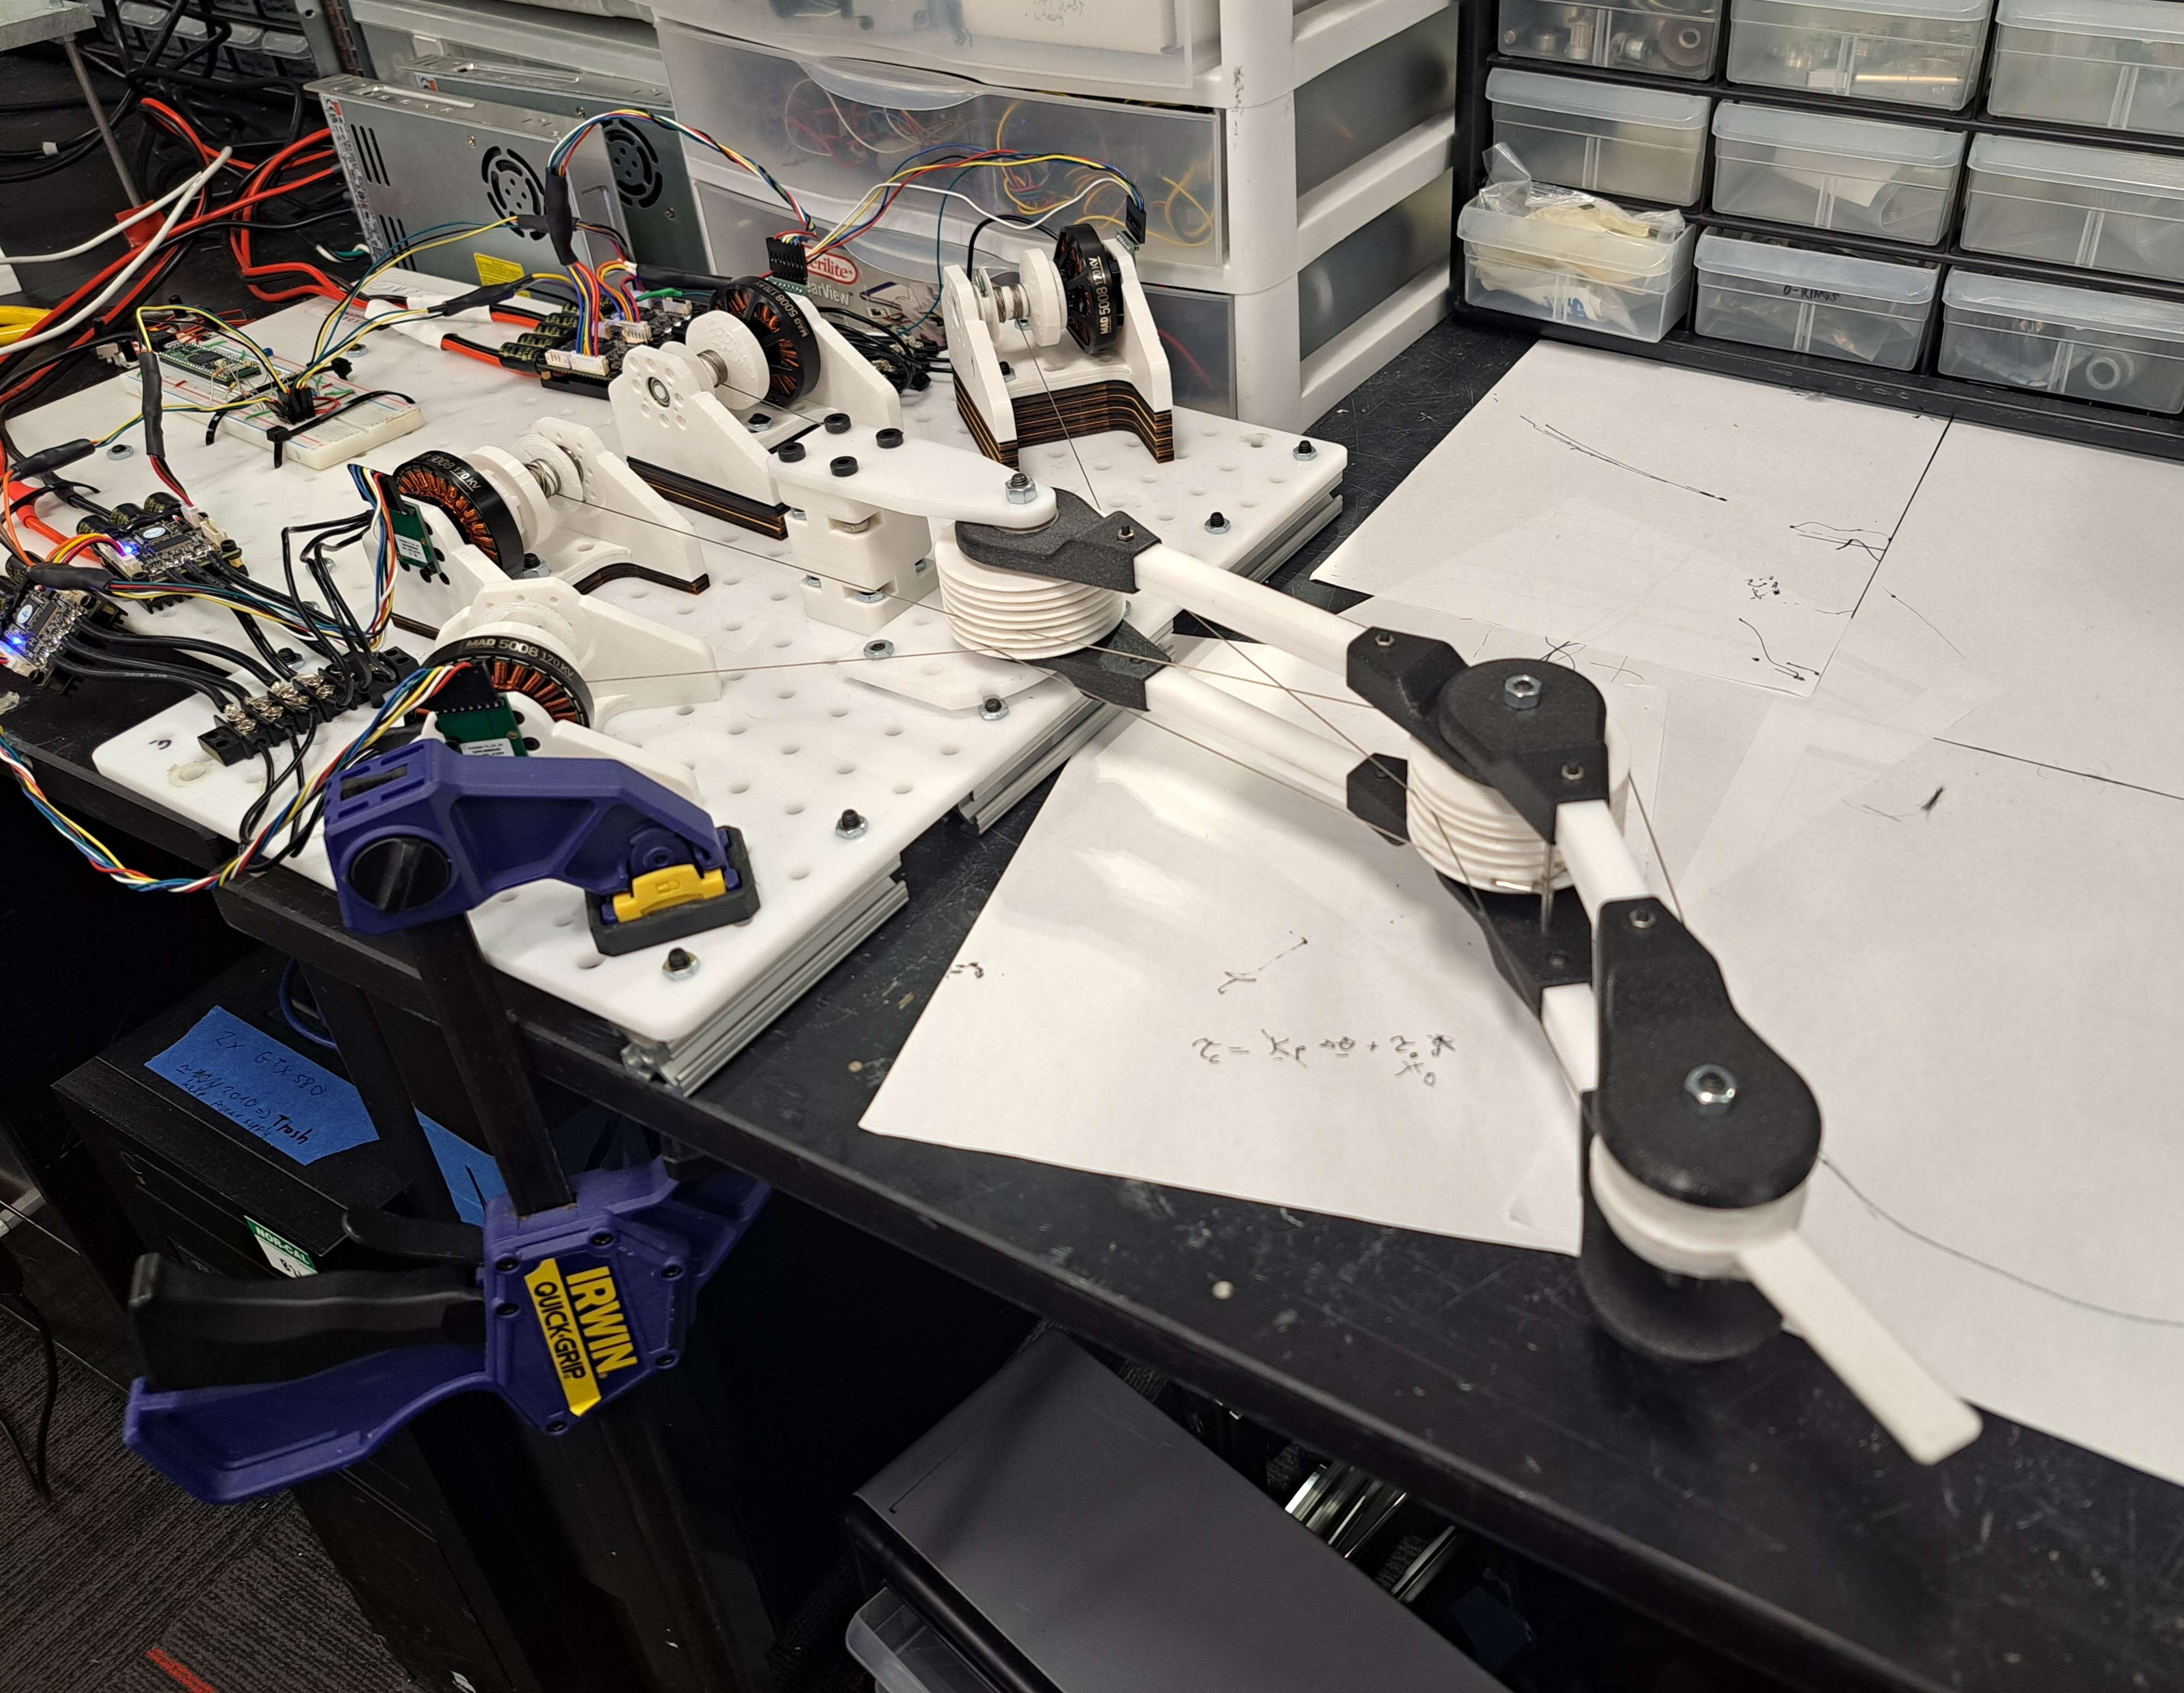
\includegraphics[width=0.8\linewidth]{testbed2_1.jpg}
\end{figure}

\newpage
\tableofcontents
\newpage

\section{Introduction}

This document aims to summarize what was done in the development and building of testbed 2, and what was learned from it, for further development with testbed 3. All of the documents related with this report, which include the software for running the arm and the can be found on this git repo and this drive. The Onshape model can be found \href{https://cad.onshape.com/documents/c940a6fae7dfa620c9d885fc/w/fe90fad0bb4f54c2b765f4a7/e/dd32a71d364b7df9178d1a8b}{here}.

\begin{figure}[H]
\centering
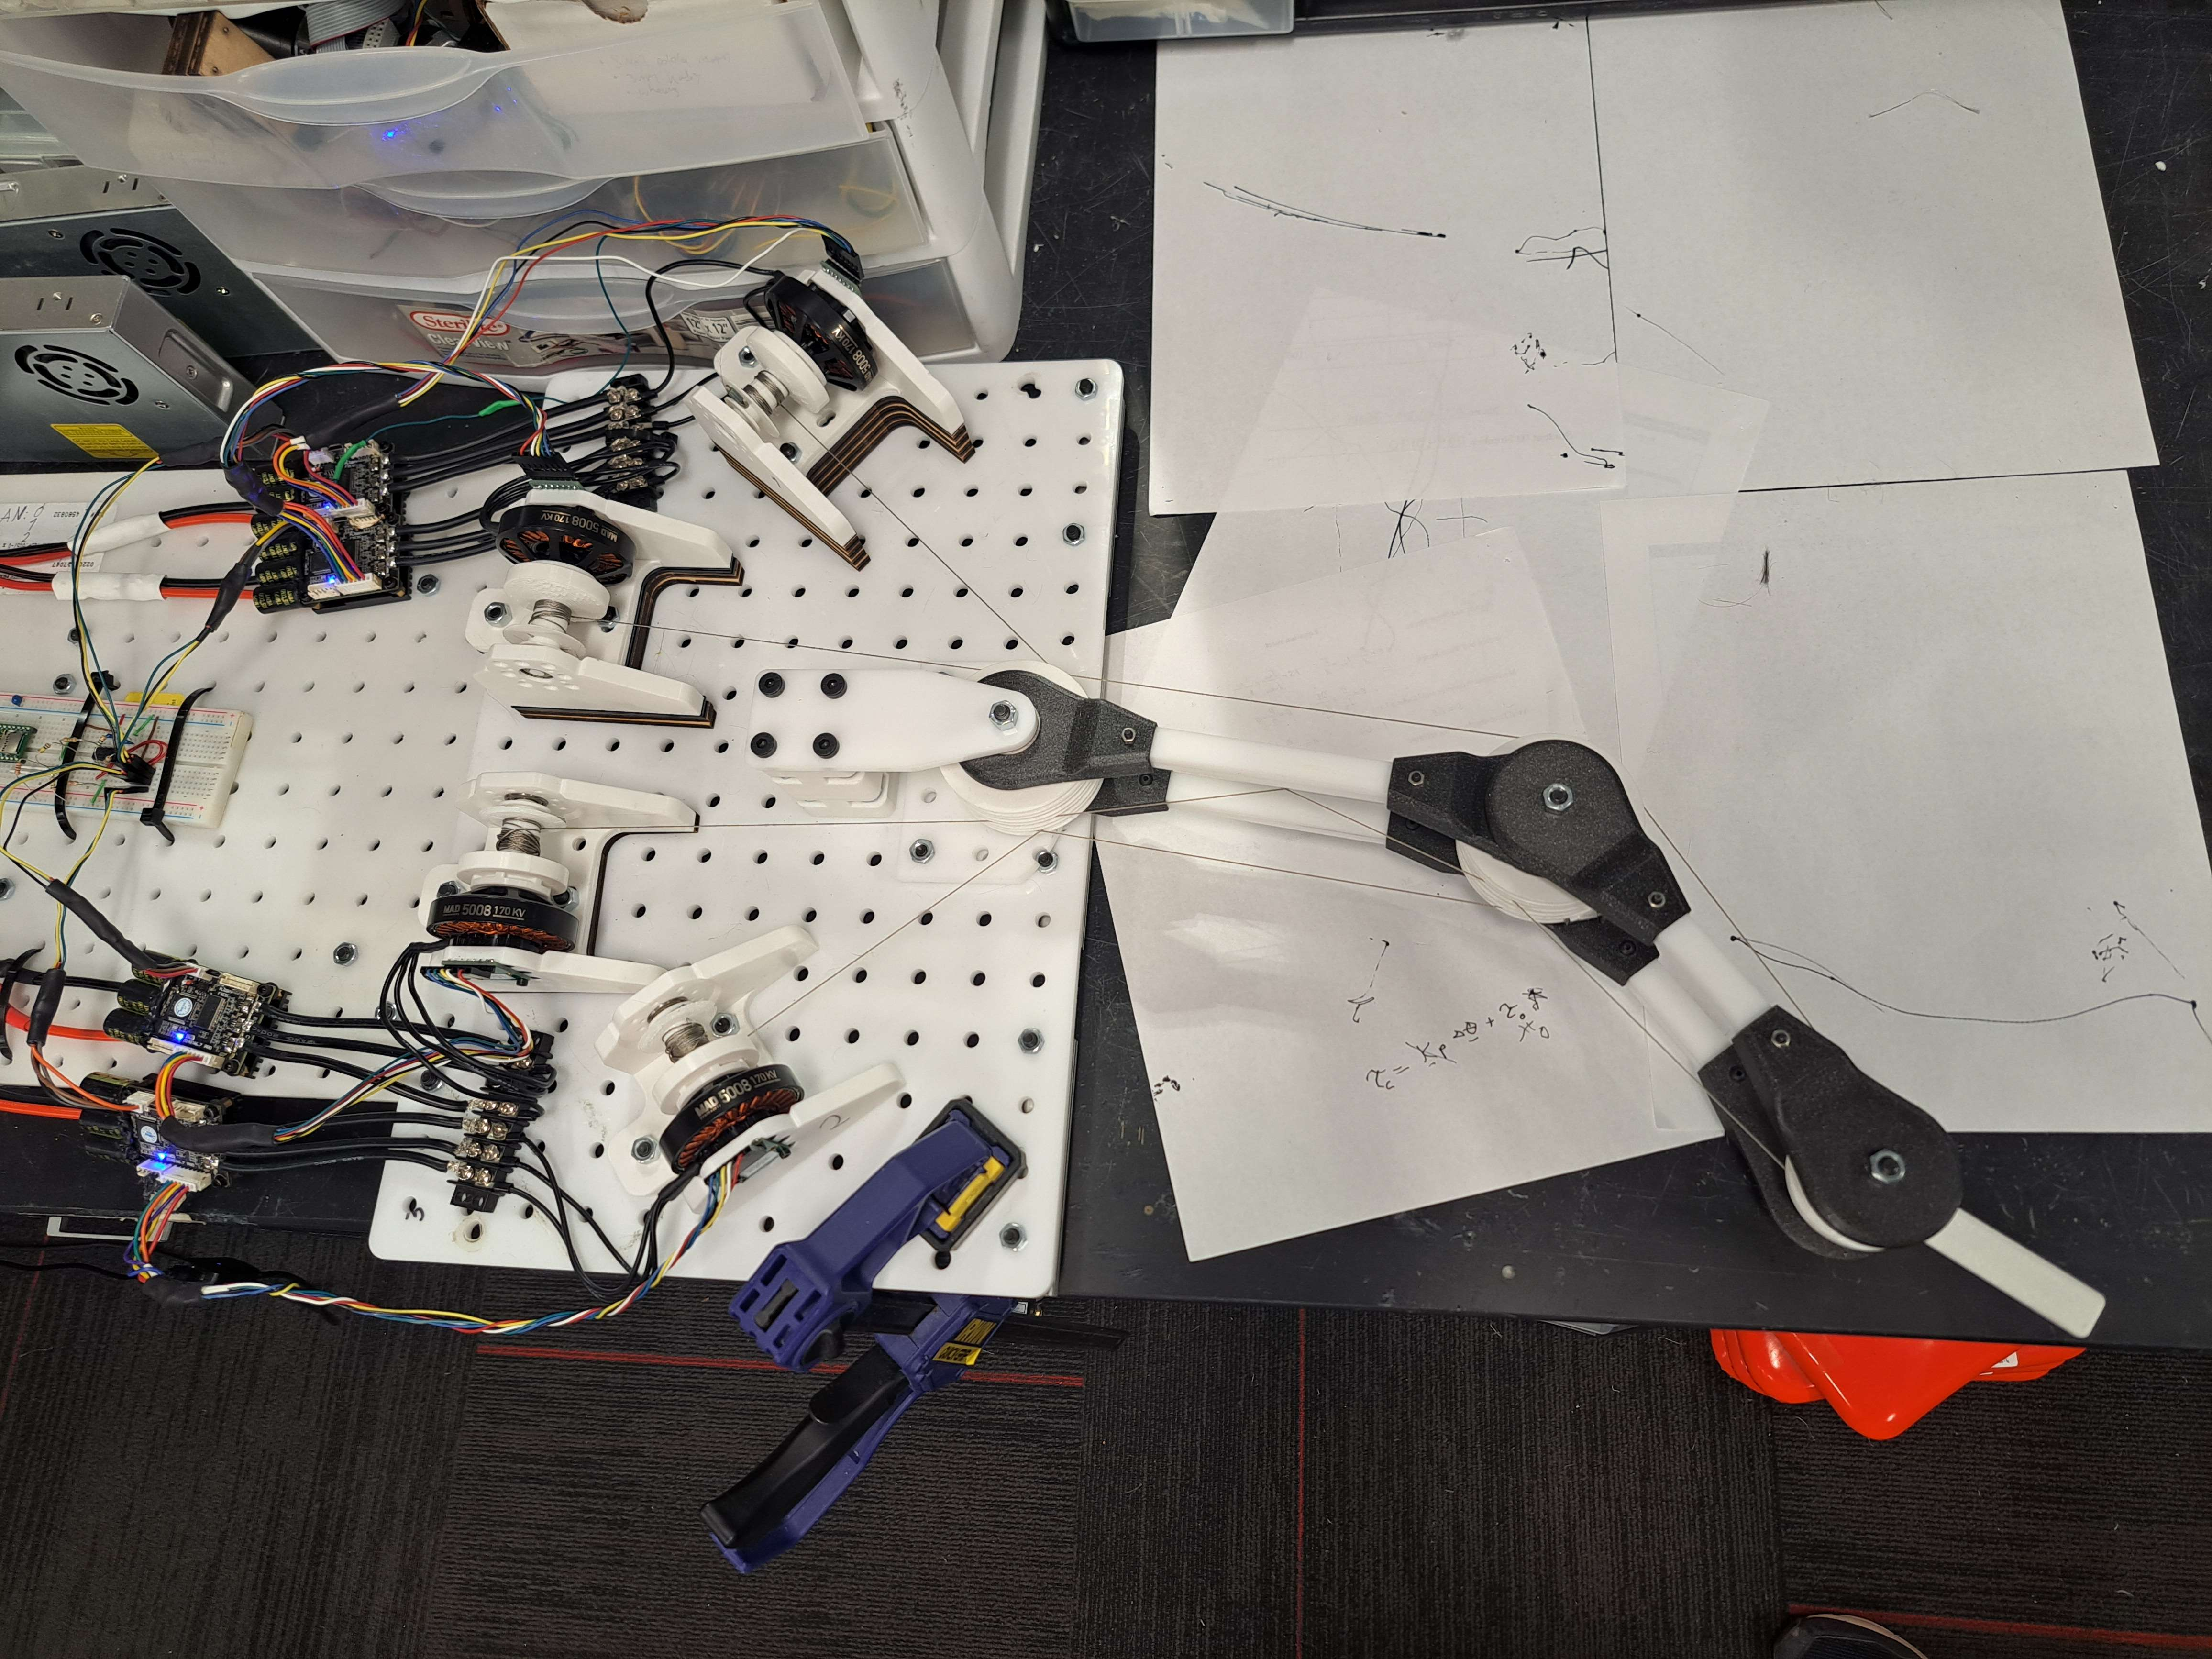
\includegraphics[width=0.7\linewidth]{testbed2_2.jpg}
\caption{\label{fig:overview}Overview of the testbed.}
\end{figure}

On the previous figure \ref{fig:overview}, we can see the testbed, with the main micro controller (partially cut on it) on  the far left, then the 4 motor drivers linked throught the CAN bus, the 4 motor pods, and then the arm with its 3 joints.


\section{Mechanical design}

\subsection{cable routing}

\begin{figure}[H]
\centering
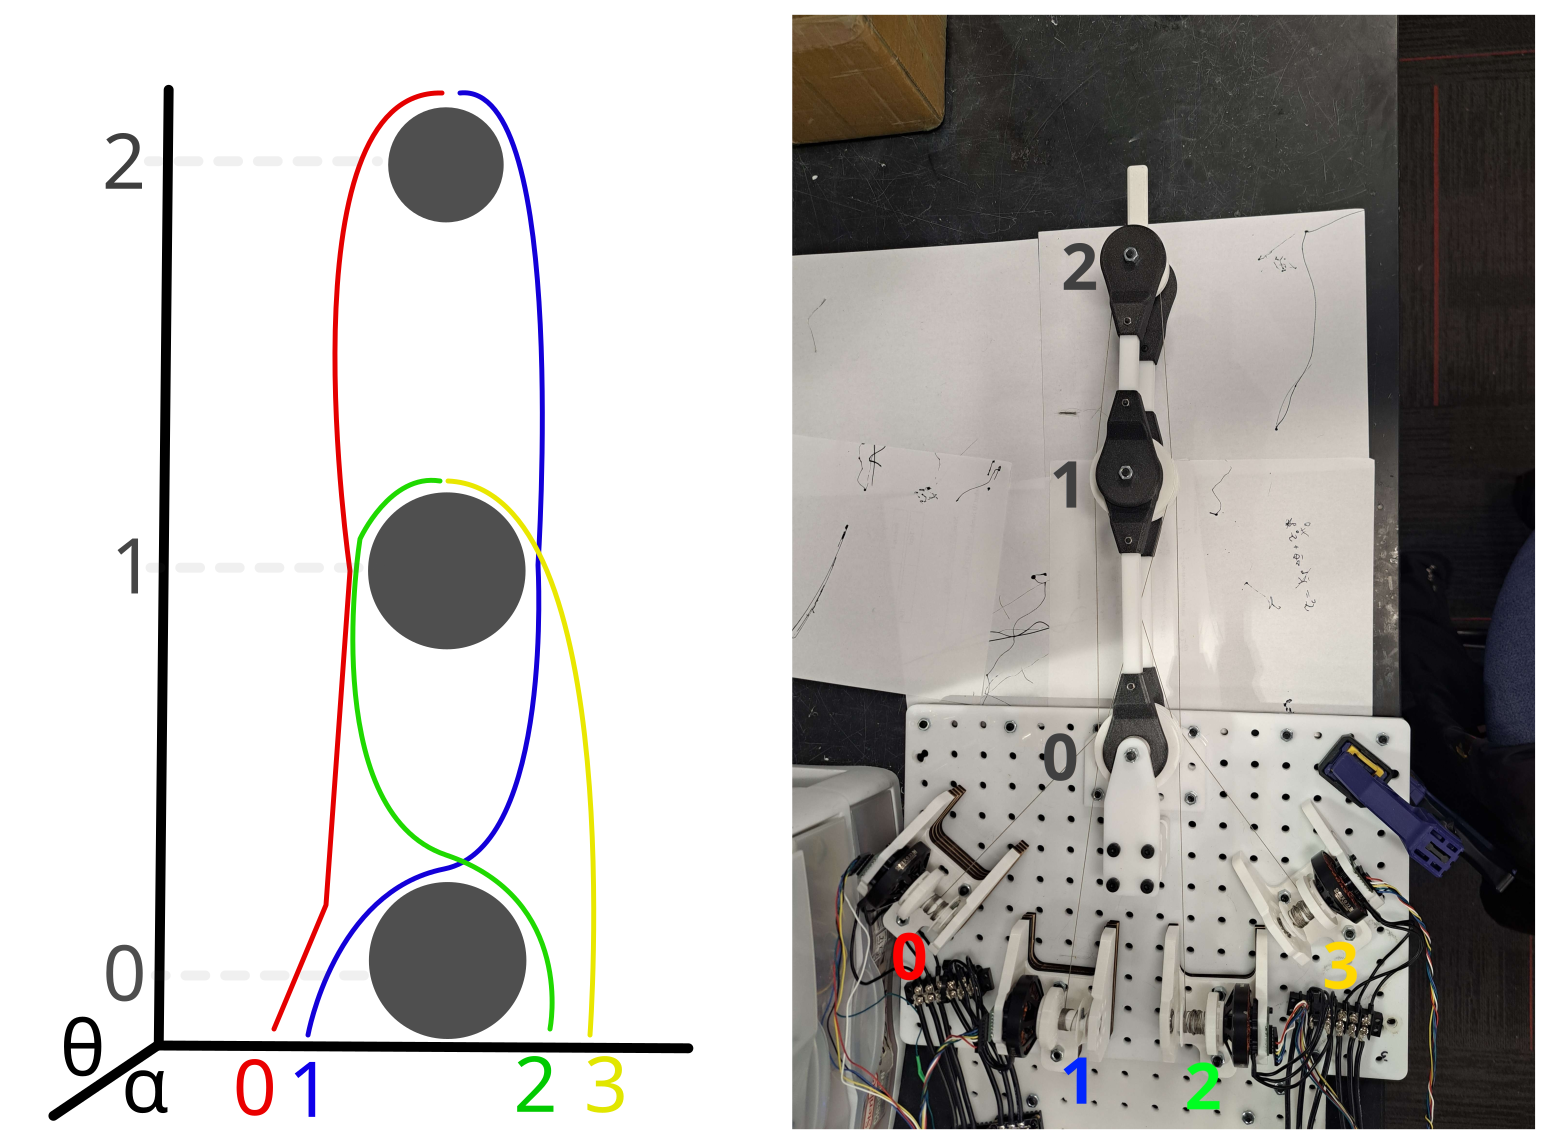
\includegraphics[width=0.7\linewidth]{cablerouting.png}
\caption{\label{fig:cablerouting}Routing of the cables in the arm.}
\end{figure}

The routing of the cables is done as shown on \ref{fig:cablerouting}. This geometry was choose for it's high degree of symmetry and hence easier control implementation features. We call the angle of each of the motors that are pulling a cable \textalpha, going from 0 to 3. We call the angle of each of the joints from the arm \texttheta, going from 0 to 2. On the actual arm, the cable linked to the motor 0 is on the top pulleys, while the cable linked to the motor 3 is on the bottom pulley. Based on \ref{fig:cablerouting}, we get that the matrix of the direction of the arm, going from \textalpha to \texttheta, is :

\begin{align}
P_{0} = \begin{pmatrix}
1 & 1 & -1 & -1 \\
1 & -1 & 1 & -1 \\
1 & -1 & 0 & 0 
\end{pmatrix}
\end{align}


Now, taking into account the diameter of the pulleys, calling $d_{m}$ the diameter of the motor pulleys and $D_{0}$, $D_{1}$ and $D_{2}$ the respective diameter of the 3 joints, we can rewrite the matrix while taking into account the reduction ratio :

\begin{align}
P = d_m \begin{pmatrix}
\frac{1}{D_{0}} & \frac{1}{D_{0}}  & -\frac{1}{D_{0}}  & -\frac{1}{D_{0}}  \\
\frac{1}{D_{1}} & -\frac{1}{D_{1}} & \frac{1}{D_{1}} & -\frac{1}{D_{1}} \\
\frac{1}{D_{2}} & -\frac{1}{D_{2}} & 0 & 0 
\end{pmatrix}
\end{align}


\subsection{sizing of the arm}

\begin{figure}[H]
\centering
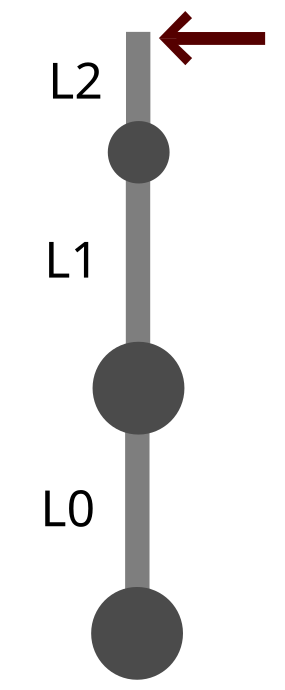
\includegraphics[width=0.1\linewidth]{linkage.png}
\caption{\label{fig:linkage}Size of the different links of the arm, and direction of the desired force capability of the arm.}
\end{figure}

To get a certain area for the arm the be able to reach, we arbitrary choose the length of the links so that the arm is about ~45cm long. We will name the length of the links $L_{0}$, $L_{1}$ and $L_{2}$. get a certain force capability $F$ at the output of the arm, we need to size the pulleys accordingly, knowing the defined length. We will name the torque capabilities of each joint $\tau_{0}$, $\tau_{1}$ and $\tau_{2}$. Finally, the torque of the motors will be named $\tau_{mi}$.
\\
First, we can write relation between $\tau_{mi}$ and the $\tau_{i}$.

\begin{align}
\frac{1}{d_{m}}
\begin{pmatrix}
D_{0} & D_{0} & -D_{0} & -D_{0}\\
0 & 0 & D_{1} & -D_{1}\\
D_{2} & -D_{2} & 0 & 0\\
\end{pmatrix}
\begin{pmatrix}
\tau_{m0} \\
\tau_{m1} \\
\tau_{m2} \\
\tau_{m3}
\end{pmatrix}
=\begin{pmatrix}
\tau_{0} \\
\tau_{1} \\
\tau_{2}
\end{pmatrix}
\end{align}

We can see a major difference between this matrix and the kinematics matrix seen above, which is that the motors 0 and 1 do moves when the second joint is rotated, but do not contribute to the torque on the second joint. This result is quiet unintuitive, but can be verified experimentally on the testbed.
To get the maximum torque of each joint, we use this relation and specify that the motors pulling in the desired direction are at $\tau_{mmax}$, and the ones from the other side are at the base co-activation $\tau_{mmin}$.


\begin{align}
\frac{2D_0}{d_m}(\tau_{mmax}-\tau_{mmin}) = \tau_{0} \\
\frac{D_1}{d_m}(\tau_{mmax}-\tau_{mmin}) = \tau_{1} \\
\frac{D_2}{d_m}(\tau_{mmax}-\tau_{mmin}) = \tau_{2}
\end{align}

Which, making the hypothesis that the co-activation is small compared to $\tau_{mmax}$ get us to :

\begin{align}
\frac{2D_0\tau_{mmax}}{d_m} = \tau_{0} \\
\frac{D_1\tau_{mmax}}{d_m} = \tau_{1} \\
\frac{D_2\tau_{mmax}}{d_m} = \tau_{2}
\end{align}


We need, if we desire to keep the arm in an equilibrium, to verify 

\begin{align}
F = \frac{\tau_{2}}{L_{2}} = \frac{\tau_{1}}{L_{2}+L_{1}} = \frac{\tau_{0}}{L_{2}+L_{1}+L_{0}}
\end{align}

Combining these equations and the precedent reasoning on the arm, we finally get that the diameters of the pulleys must verify :

\begin{align}
D_2 &= \frac{F d_mL_{2}}{ \tau_{mmax}} \\
D_1 &= \frac{F d_m(L_{2}+L_{1})}{ \tau_{mmax}} \\
D_0 &= \frac{F d_m(L_{2}+L_{1}+L_{0})}{2 \tau_{mmax}}
\end{align}

And we see that all of the 3 pulleys are proportional to the diameter of the motor pulleys. The motor pulleys diameter can be choose arbitrarily, but its final value will change the tension of the cables. Bigger motor pulleys will mean relieving the cables from some stress, but also that the value of the $D_{i}$ will be bigger, which can be inconvenient for the size of the arm. The final choice was to made these pulley quiet small.

\vspace{0.5cm}
Now we know that $\tau_{mmax}$ is about 1N.m for a motor, that $L_0=21cm$, $L_1=16cm$, $L_2=9cm$ and that $d_m=1.4cm$.
The target force that we want is about 16N of force. We could go for a bigger force and hence reduction ratio, but that would lead to a high refleted inertia of the motor to the arm). With all of that, we get that $D_2 = 2cm$, $D_1=5.6cm$ and $D_0=5.2cm$. These value were in the end rounded to $D_2 = 3cm$, $D_1=6cm$ and $D_0=6cm$, ensuring that we get the desired force capability.

\subsection{Building of the testbed}
The testbed was designed entirely on Onshape, the project can be found \href{https://cad.onshape.com/documents/c940a6fae7dfa620c9d885fc/w/fe90fad0bb4f54c2b765f4a7/e/dd32a71d364b7df9178d1a8b}{here}.
The testbed was build using mostly 3D printed PLA, and lasercutting of Delrin and Plexiglas for some parts (using the laser cutter from lab64). This was because of the convenience of using already mastered tools for me, instead of going for more rigid aluminum. I would say it's fine for what we are doing with this testbed right now.

\begin{figure}[H]
\centering
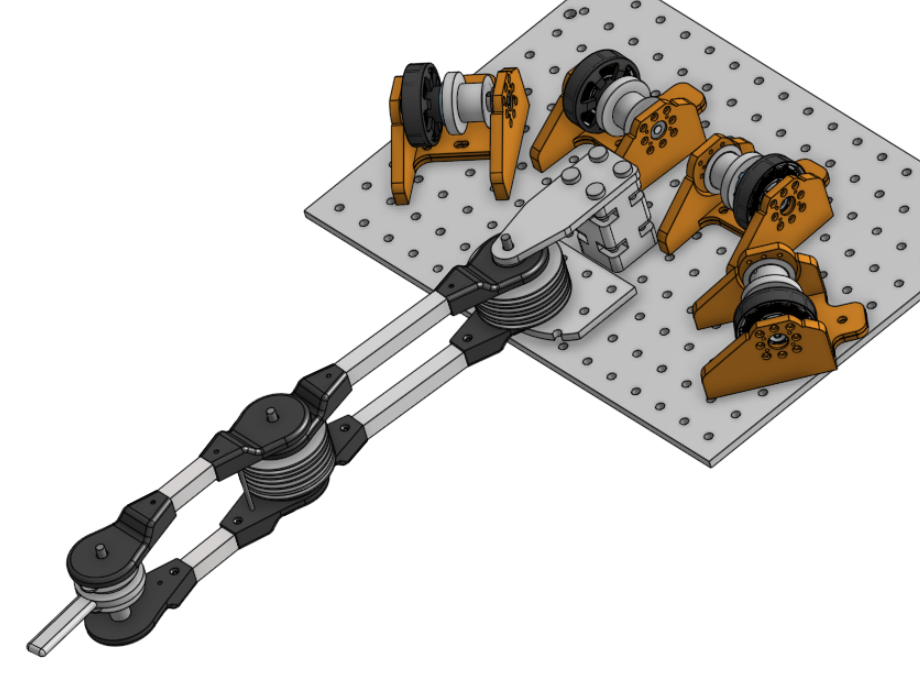
\includegraphics[width=0.5\linewidth]{Onshape.png}
\caption{\label{fig:Onshape}Onshape model.}
\end{figure}

\subsection{What to improve mechanically for testbed 3}

\begin{itemize}
\item Design a structural link between the top and the bottom part of the arm to improve it's rigidity by a lot (see the blue lines on \ref{fig:pulleysideview}).
\item Switch to aluminum for parts that handle a lot of load and can bend due to it (You can use sendcutsend or JLCCNC for machining them if necessary, it is not that expensive if the part is designed properly). Some of the parts that were bending a lot were especially on the motor side, like the main plate that was made out of flexible Plexiglas, and the motor pulley as well. For the motor pulley, putting a Dowel pin in it may do the trick for making it more rigid.
\item Switch to a spiral drum and spiral pulleys to prevent cables from ripping against each other. The current smooth pulleys and drums lead to some undesired behaviors, long term tear off of the cable and awful noises. This may be a not so good idea if the arm pulleys ends up being taller, making the arm too tall compared to its width.
\item switch from steel cables to dyneema cable.
\item We can merge two of the pulleys from the second joint (the ones circled in red on \ref{fig:pulleysideview}) into one, as their movement are already linked anyway. This reduce the part count and complexity of the arm by a bit. What to get from this is that one pulley per cable is not necessary if adjacent pulleys ends up having a linked rotation in the same direction anyway.
\end{itemize}

The next mechanical challenges to solve on testbed 3 nest in how to run the cables in a non-planar arm.

\begin{figure}[H]
\centering
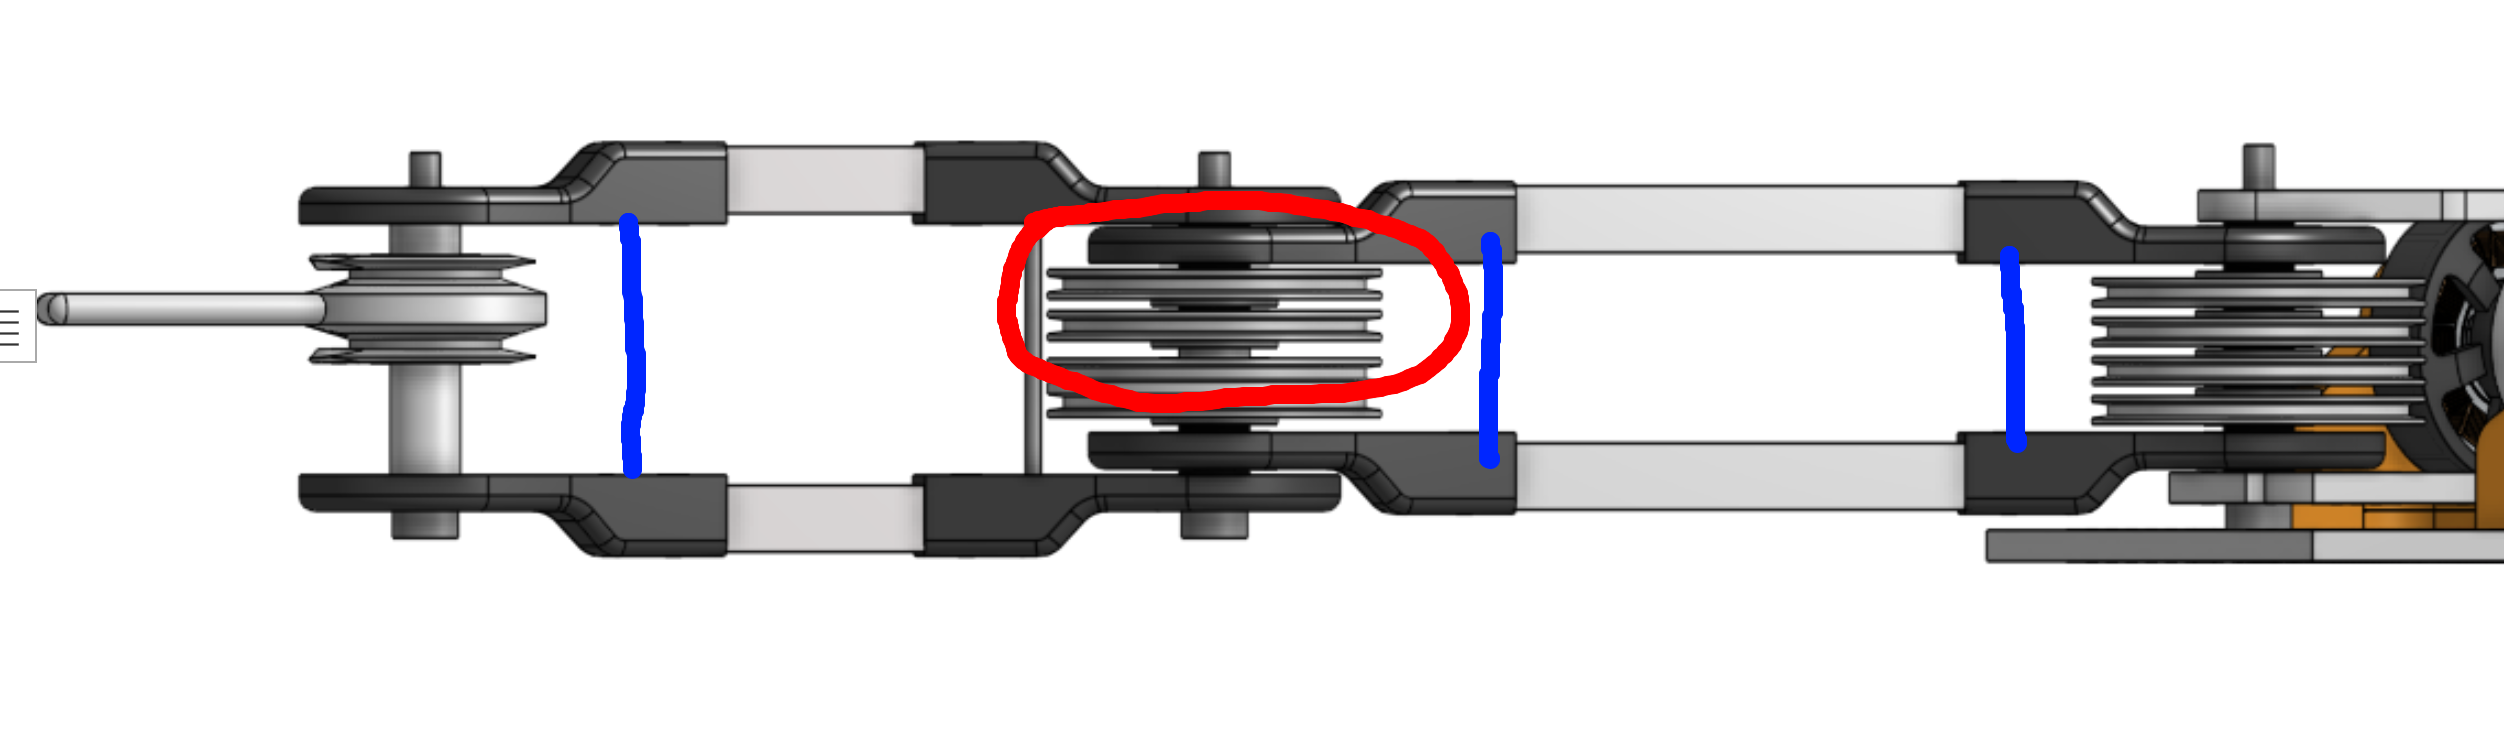
\includegraphics[width=0.8\linewidth]{pulley sideview.png}
\caption{\label{fig:pulleysideview}Sideview of the arm on Onshape.}
\end{figure}

\begin{figure}[H]
\centering
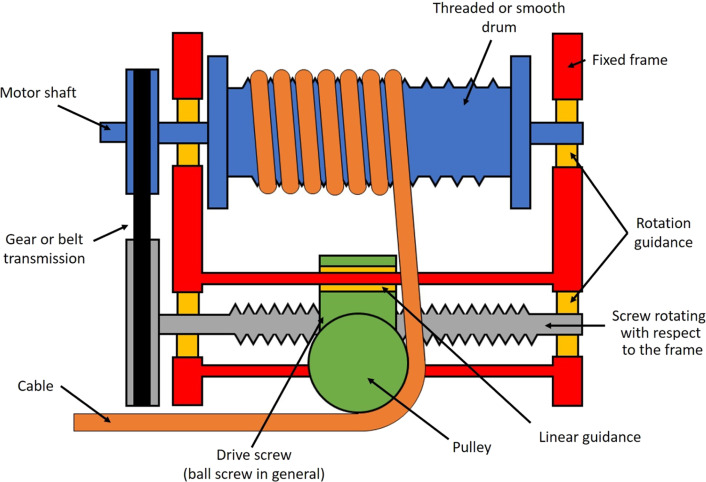
\includegraphics[width=0.3\linewidth]{spiraldrum.jpg}
\caption{\label{fig:spiraldrum}An example of an interesting way to make a spiral drum. Doing it this way can also enable a permanent pretensioning of the cables by adding a spring in the system.}
\end{figure}


\section{Electrical design}

\subsection{General architecture}

\begin{figure}[H]
\centering
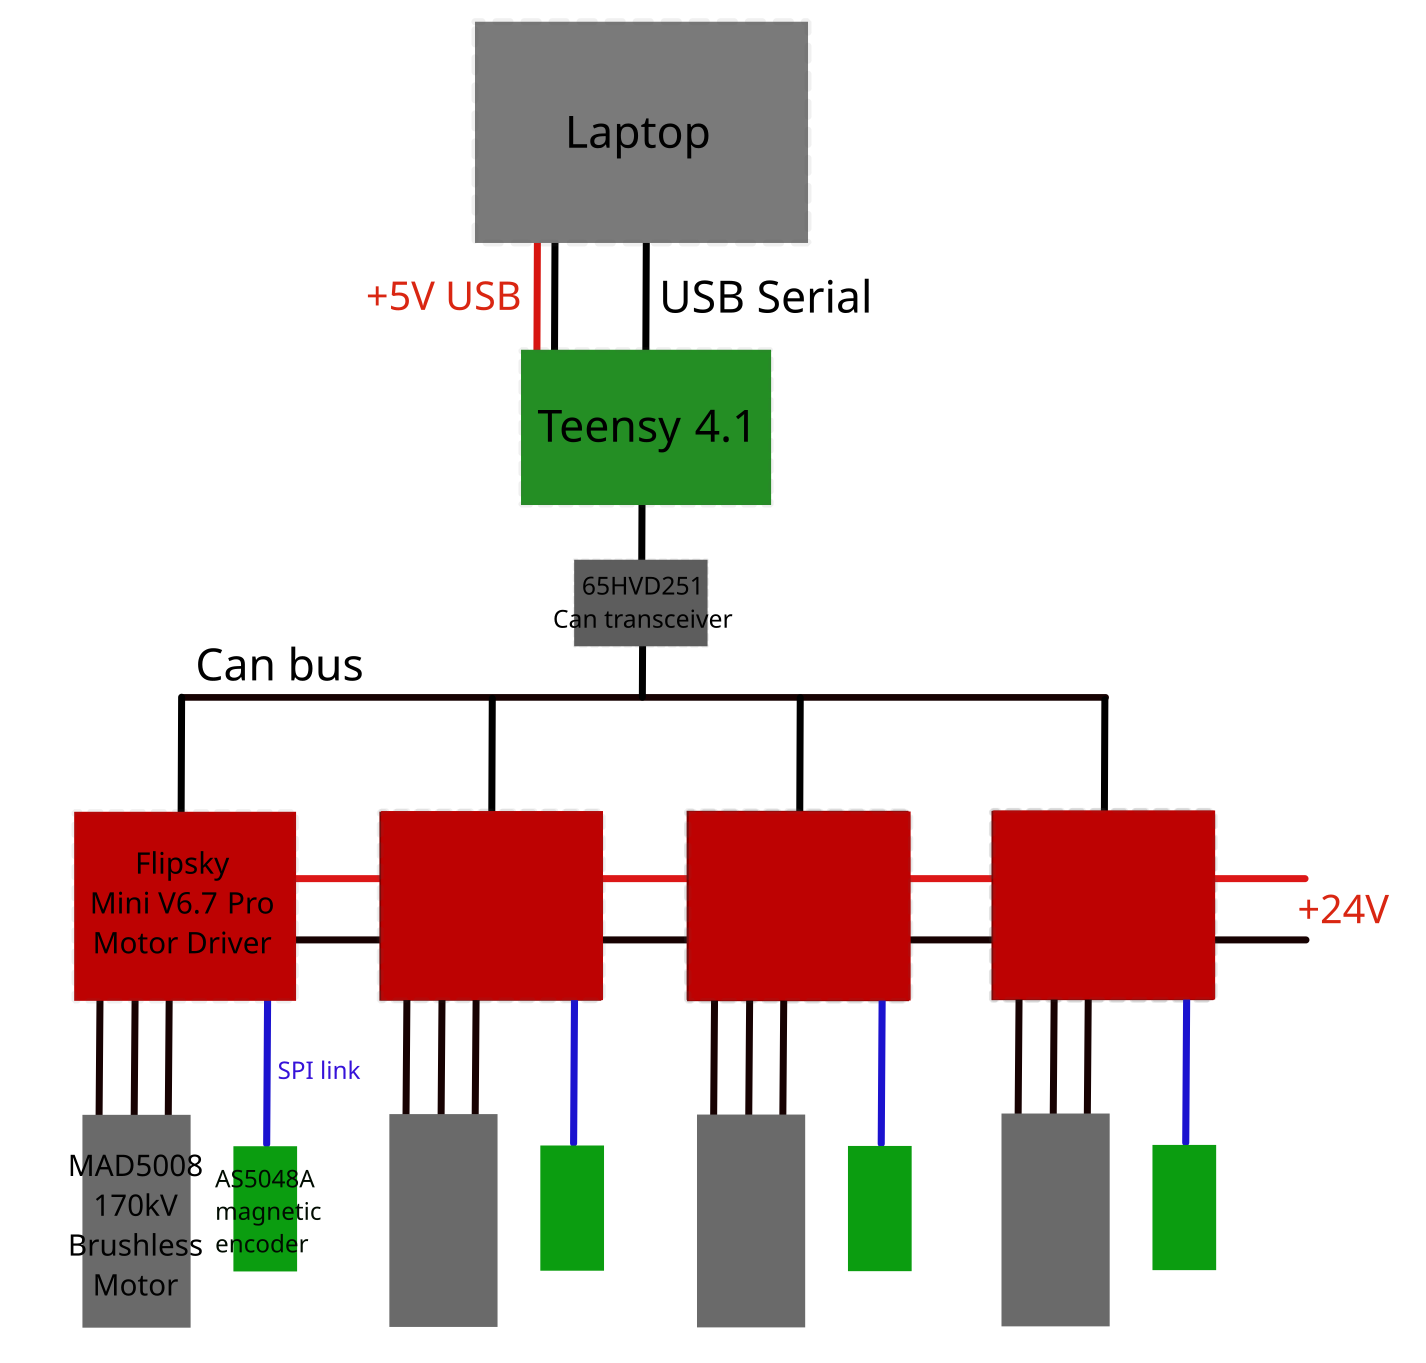
\includegraphics[width=0.7\linewidth]{elec.png}
\caption{\label{fig:elec}Architecture of the electronics of the arm.}
\end{figure}

To power on the testbed, you need to plug in the two 24V power supplies that power the motor drivers, and then plug in the usb cable coming from the Teensy to your computer.

\subsection{references of the components}

\begin{itemize}
    \item \href{https://www.pjrc.com/store/teensy41.html}{Teensy 4.1} (a great and powerful microcontroller)
    \item \href{https://www.digikey.com/en/products/detail/texas-instruments/SN65HVD251P/948551}{SN65HVD251 Can tranceiver}
    \item \href{https://flipsky.net/products/mini-fsesc6-7-pro-70a?variant=42664011956465&country=US&currency=USD&utm_medium=product_sync&utm_source=google&utm_content=sag_organic&utm_campaign=sag_organic}{FLIPSKY Mini FSESC6.7 PRO motor driver}
    \item \href{https://mad-motor.com/products/mad-components-5008-eee?VariantsId=10441}{5008 EEE 170kV MAD brushless motor}
    \item \href{https://www.digikey.com/en/products/detail/ams-osram-usa-inc/AS5048A-ADAPTERBOARD/3188612}{AS5048A magnetic encoder}
\end{itemize}

\subsection{The motor drivers}

One of the main wrong choice that was made was to use Flipsky motor drivers (that are originally meant for powering skateboard motors). They indeed can drive brushless motors with field-oriented control, but this choice led to needing to change the resistors on the motor drivers, and unsoldering them is a painful process to do (and is risky for the driver, you can damage it doing so). For better current capabilities, it was needed to switch from $0.005\Omega$ resistors to $0.05\Omega$ ones.

\begin{figure}[H]
\centering
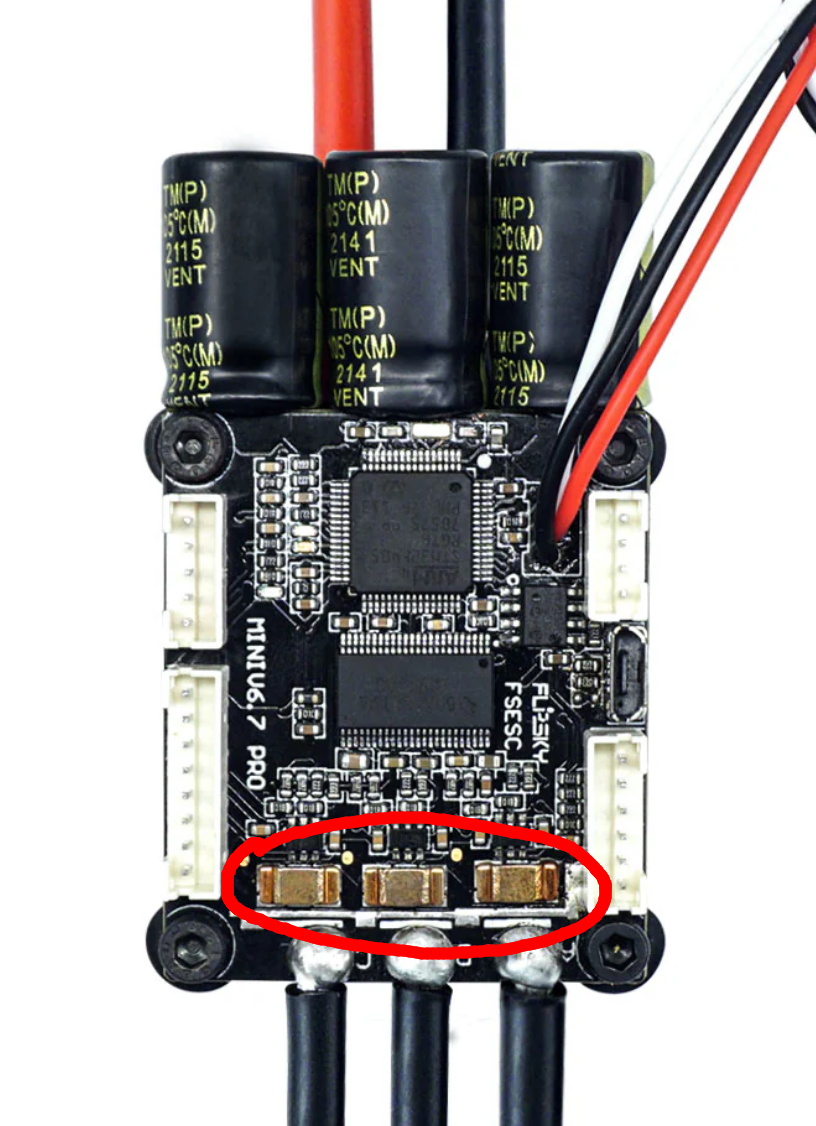
\includegraphics[width=0.4\linewidth]{Motordriver.png}
\caption{\label{fig:motordriver}The motor driver, with the resistors circled in red.}
\end{figure}

\subsection{Electrical tips for testbed 3}
\begin{itemize}
\item To get a better data rate and less interruption during the control loop due to Serial transmission to the laptop (which is quiet slow), it may be interesting to buy a CAN to USB module to make the laptop communicate directly throught the CAN bus, enabling us to get much more data in real time. It may also introduce more complexity in terms of coding, so I'm not totally sure about the pertinence of doing it for now.
\item for discussion about choosing a new motor driver and new motor, see the chapter on Cogging.
\end{itemize}
\newpage
\section{Software}

The framework used for the development this testbed software was PlatformIO on VSCode. I recommend finding a quick tutorial on it to learn about it, how to upload a code, look at the Serial Monitor, ect...
You also need Python for the computer interface.
The current code is made so that you can extend it as much as you like for high number of degrees of freedom, as long as you take the time to write down the invert kinematics matrix, and change the Controlloopcallback function. This should enable a rapid iteration on the code for the next testbed.
\\
\vspace{0.1cm}

To upload a new code on the Teensy 4.1, you can directly plug it to your computer with a micro-USB cable. For the motor drivers, it's a little trickier, as you need to use an external JTAG uploader. The one that we're using is the one from the white nucleo board on \ref{fig:nucleoboard}. To plug it to a motor driver, just plug the 5-pins cables to the motor driver. You can then upload a new code to the motor driver throught it. One thing to take care of when doing so is to change the CAN address of the driver written in the code to the corresponding one (the number of the motor, from 0 to 3, being the CAN address of the motor driver you are uploading to).
\\

Reading this, you should have understand that the software from the testbed is made of two main parts : the code for the Teensy main micro controller, and the code for all of the drivers.

\begin{figure}[H]
\centering
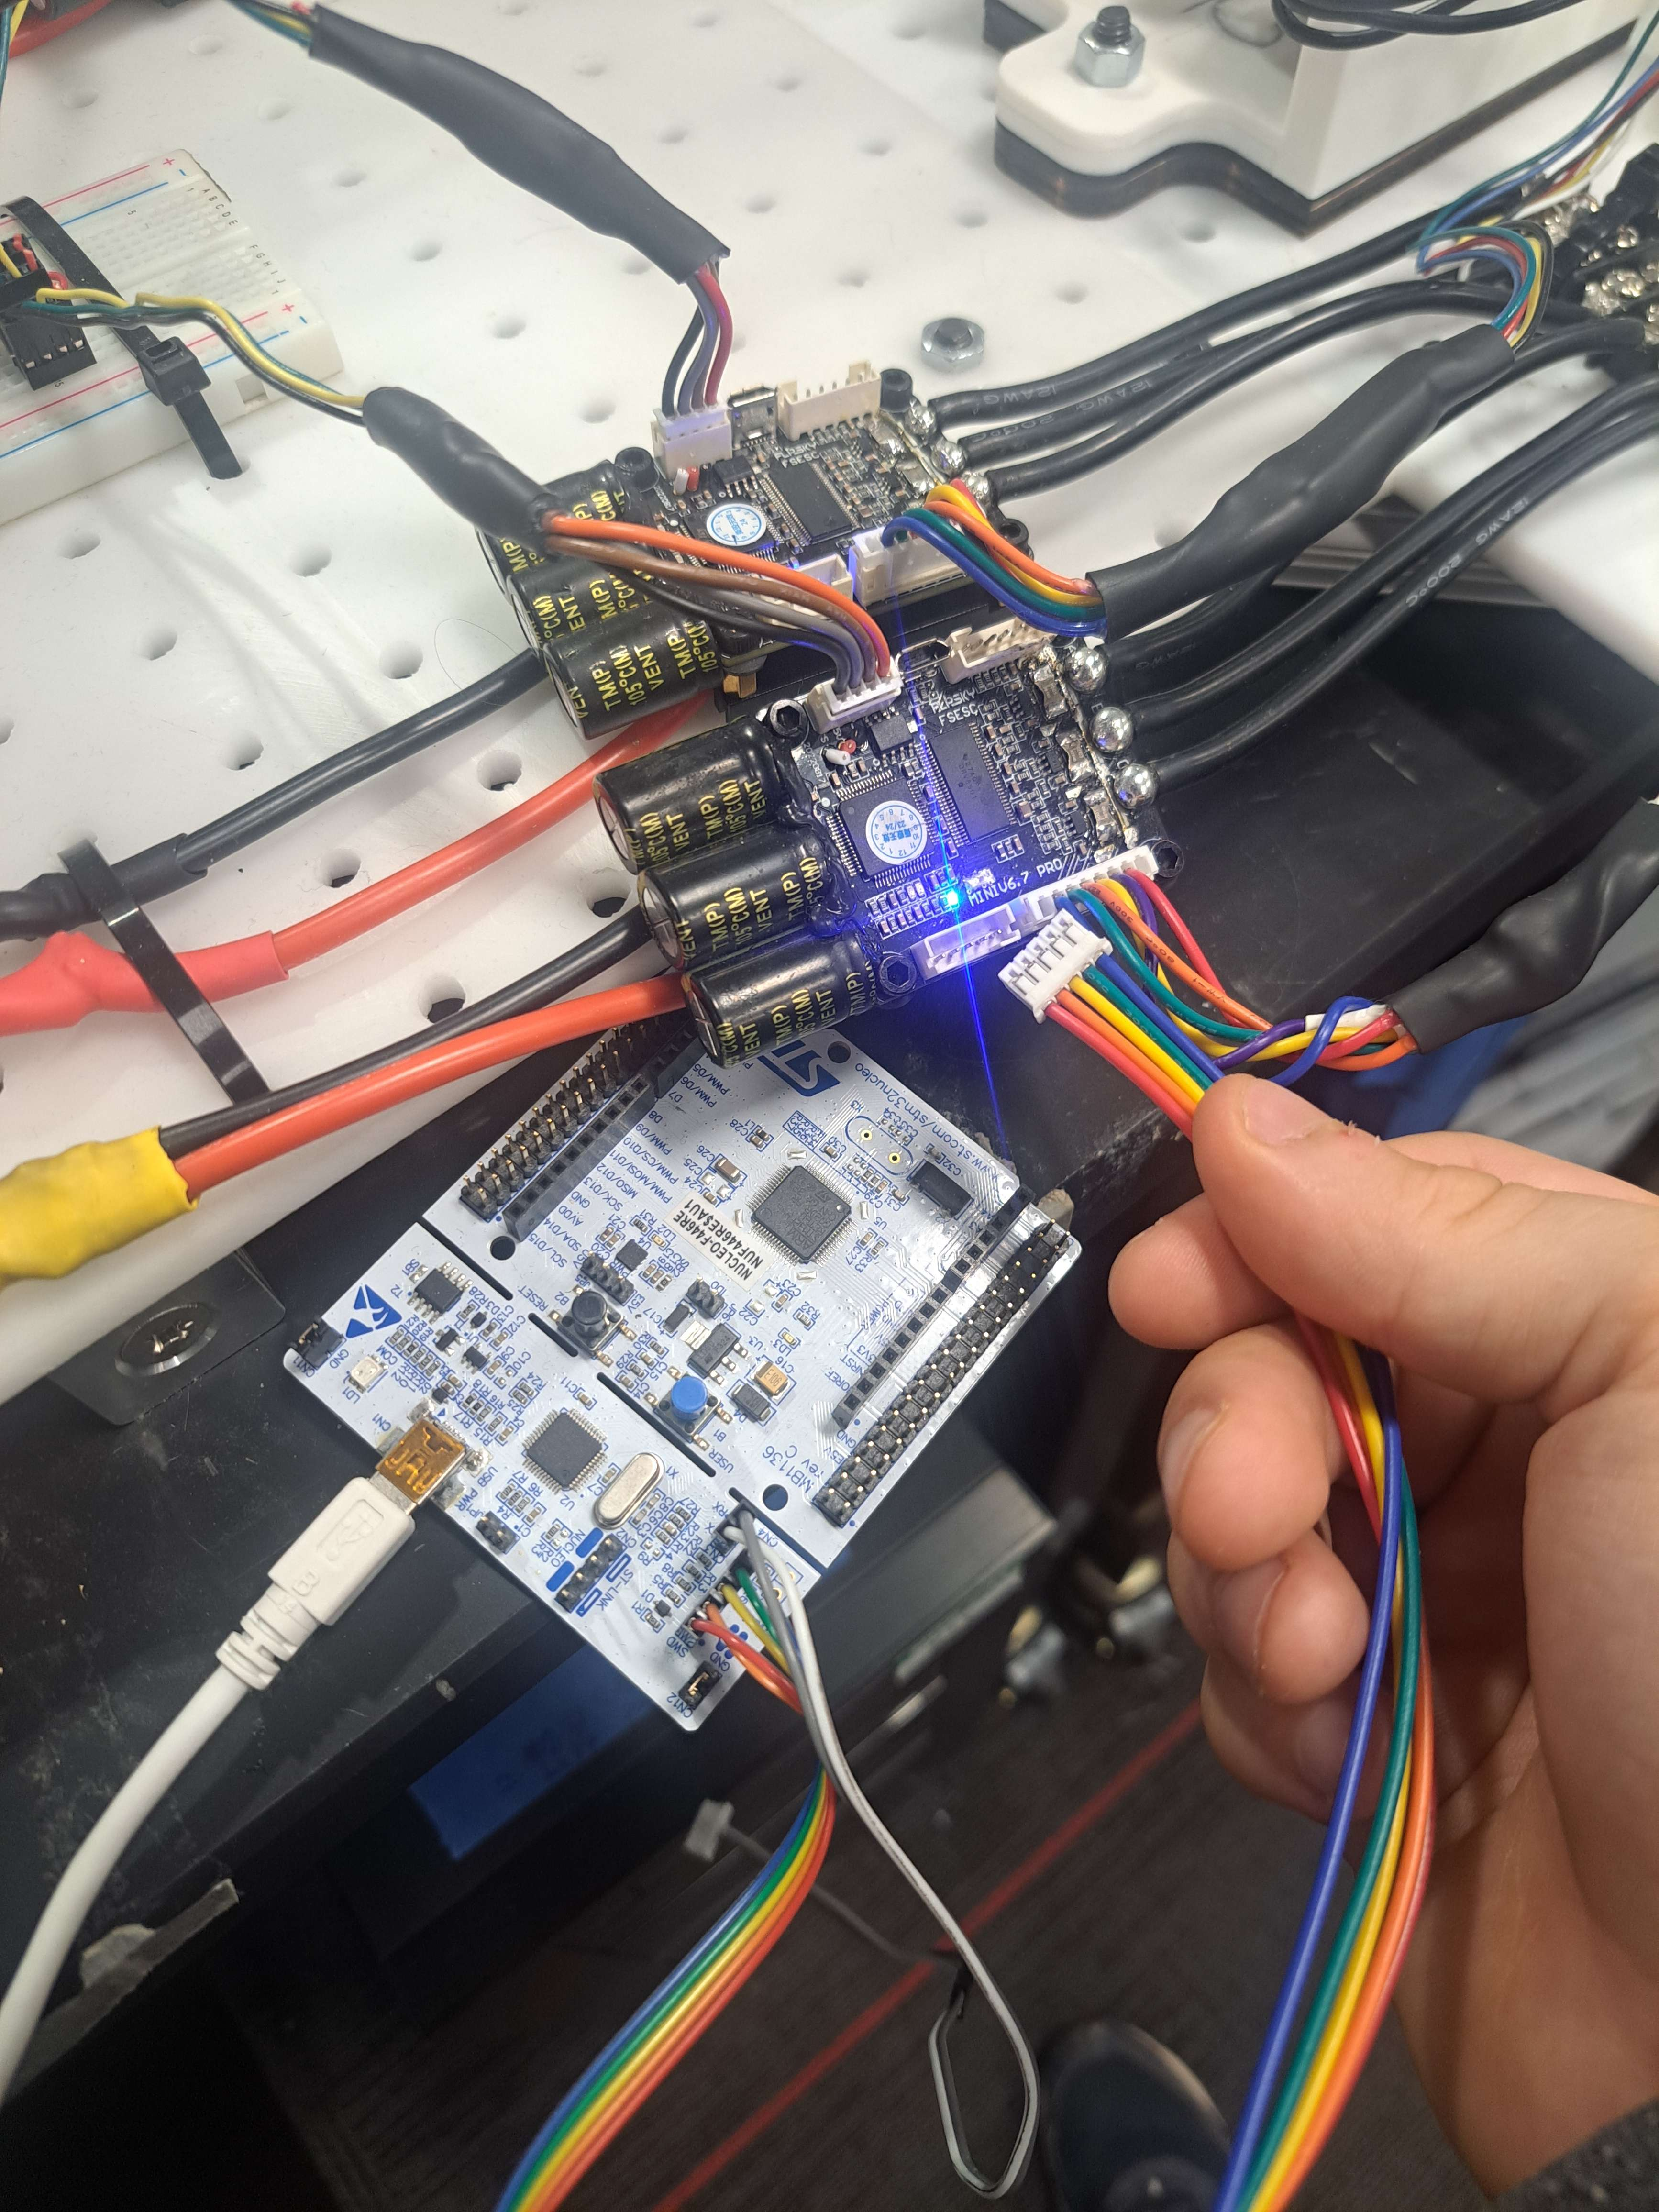
\includegraphics[width=0.3\linewidth]{Nucleoboard.jpg}
\caption{\label{fig:nucleoboard}The 5 pins connector to plug and the white nucleo board.}
\end{figure}

\subsection{Teensy code}

\subsubsection{TaskScheduler}

The main code running on the Teensy is heavily based on the TaskScheduler library. This library allows us to specify a frequency for the execution of several functions in a simple and readable way, as long as the micro controller has the processing power to respect the specified timings.

\begin{figure}[H]
\centering
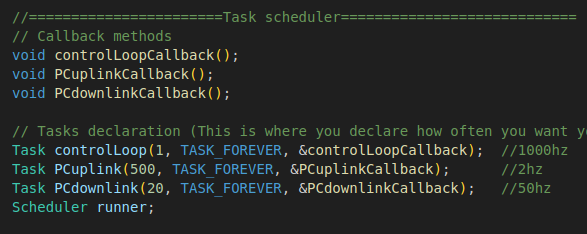
\includegraphics[width=0.6\linewidth]{Taskscheduler.png}
\caption{\label{fig:tasksched}The task scheduler functions declaration.}
\end{figure}

We call the functions that we want to call "Callback", and in the Task declaration we specify the delay to happen between each execution of the function. For example, the controlLoop is called once every millisecond, the PCuplink once every 500ms and the PCdownlink once every 20ms (equivalent to 1000Hz for the controlloop, 2Hz for sending back monitoring datas to the PC and 50Hz for processing messages incoming from the PC).

\subsubsection{CAN bus and objects}

Another main point of this code is how to the CAN bus is managed. It's managed using objects named FOCDriver that are the image of the motors drivers from the Teensy point of view. The Teensy is the master of the CAN bus, starting every communication on it. It can either use a set method to send a value to one of the driver to be set on it, or a get method that asks for an update of a value that is currently stored in the object.
\\
In the driver code, a Controller object is the image of the Teensy, and it handles the reception of these set and update, and in the case of the later send back the requested value.
\\
One the drawback of the way the CAN bus is managed is that you need to call processCANMessages that manage the reading of the incoming message often to ensure that any received new information is handled as soon as possible. In reality it could be improved if you call the function only when you know that there should be a new CAN message (because the Teensy initiate any CAN communication, you're able to predict when a new message should be there). But I didn't did it and instead decided to call calling the processCANMessages often in the different functions. It works so why changing it.

\subsection{Driver code}

The driver code essentially execute a FOC-oriented control algorithm on the motor driver. The principle of FOC is, using the phase currents and the position of the motor, to enable precise torque control of the motor. For that, we're using the \href{https://docs.simplefoc.com/}{SimpleFOC} library that I recommend you to read the documentation.

\begin{figure}[H]
\centering
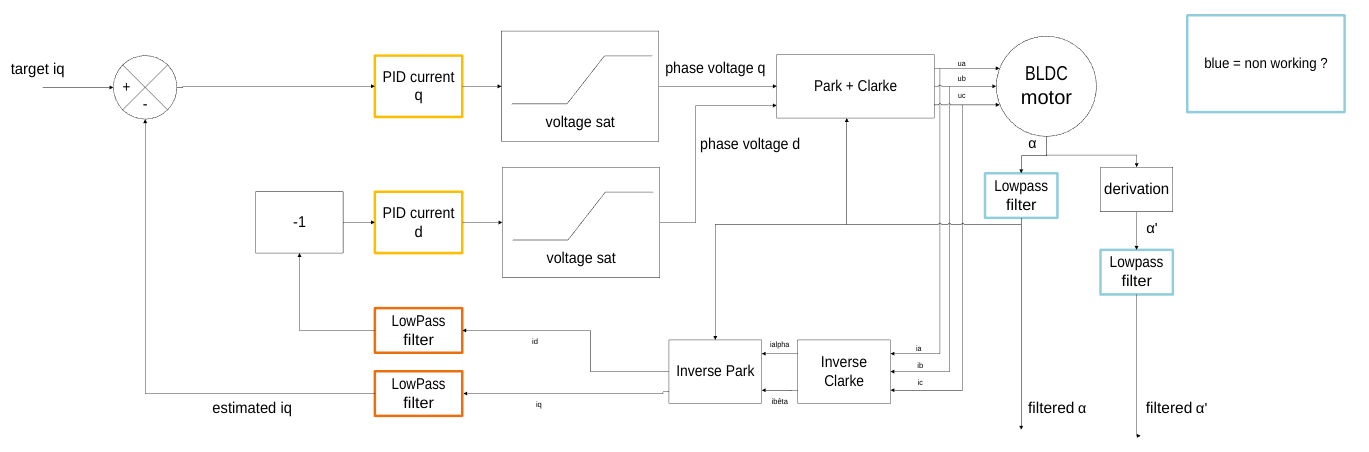
\includegraphics[width=0.8\linewidth]{FOC.png}
\caption{\label{fig:FOC}The FOC algorithm executed on the driver.}
\end{figure}

\newpage
\section{Control}

All the $\theta$ are 3-dimensional vectors in the joint space, and all of the $\alpha$ are 4-dimensional vectors in the motor space. Iq is 4-dimensional as well, and is actually named targetforce in the code.

\subsection{Torque control}

\begin{figure}[H]
\centering
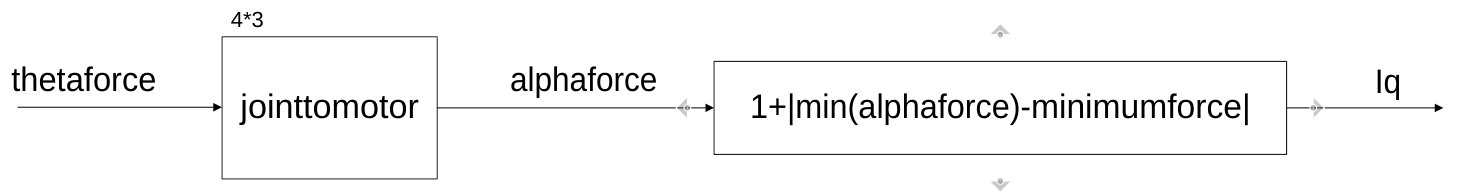
\includegraphics[width=0.8\linewidth]{torquecontrol.png}
\caption{\label{fig:torquecontrol}The torque control algorithm executed on the Teensy}
\end{figure}

The torque control algorithm is quiet straigthforward, with one subtility being the way the coactivation is calculated. The principle of the coactivation is to look which motor has the minimal torque that will be applied to it (which is generally negative) and to increase it until this particular motor has a minimalforce applied it so it keeps the cables tensioned. You then also increase the force applied by all the other motors by the same amount, so that there's no bias in the output torque of the arm.
\\
The current Python interface of the torque control algorithm is a small interface with 4 sliders to command the torque of the 3 arm joints + the coactivation. A cool demo to do with this code is simply to let the torque to be 0 on all of the joints and move the arm freely by hand, while all of the cables stay tensionate, you can quiet feel the motor through the transmission.
\vspace{0.1cm}
\\
The jointtomotor function is the following matrix product : 

\begin{align}
P = d_m \begin{pmatrix}
\frac{1}{D_{0}} & \frac{1}{D_{1}}  & \frac{1}{D_{2}} \\
\frac{1}{D_{0}} & -\frac{1}{D_{1}} & -\frac{1}{D_{2}} \\
-\frac{1}{D_{0}} & \frac{1}{D_{1}} & 0 \\
-\frac{1}{D_{0}} & -\frac{1}{D_{1}} & 0 \\
\end{pmatrix}
\begin{pmatrix}
\tau_{0} \\
\tau_{1} \\
\tau_{2}
\end{pmatrix}
=\begin{pmatrix}
\tau_{m0} \\
\tau_{m1} \\
\tau_{m2} \\
\tau_{m3}
\end{pmatrix}
\end{align}

\subsection{Position control}

\begin{figure}[H]
\centering
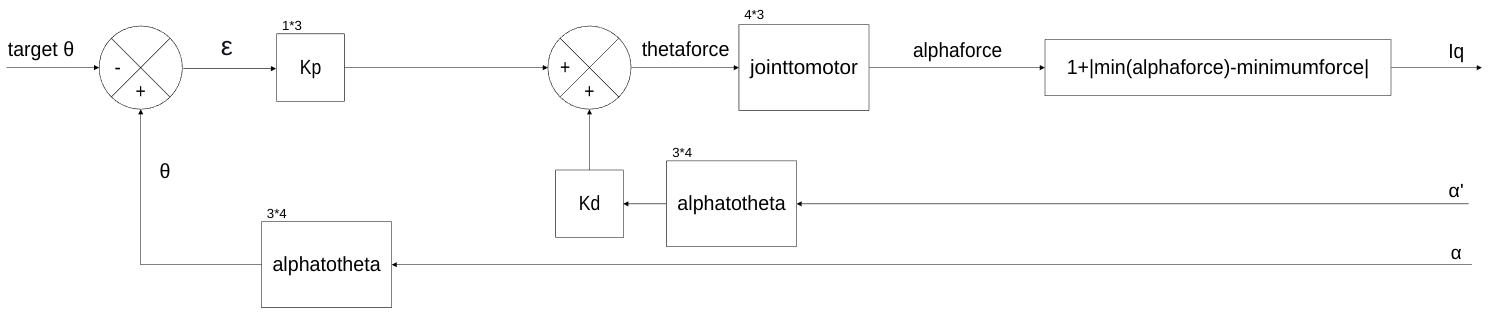
\includegraphics[width=0.8\linewidth]{positioncontrol.png}
\caption{\label{fig:poscontrol}The position control algorithm executed on the Teensy}
\end{figure}

The position control loop reuse the torque control algorithm and use the position and speed measurements made on each of the motors to implement a PD control loop, in $\theta$ space. There is thus 3 Kp and 3 Kd values, one for each joint. Their current values were roughly choose at the end of my stay in the lab and could be finetuned, first by being leveled so that the joint-to-joint transmission feel more natural, and then by being increased or decreased so that the arm is either stiffer or more compliant.

The alphatotheta function is the following matrix product : 

\begin{align}
P =  \begin{pmatrix}
\frac{d_m}{4D_0} & \frac{d_m}{4D_0} & -\frac{d_m}{4D_0} & -\frac{d_m}{4D_0} \\
0 & 0 & \frac{d_m}{2D_1} & -\frac{d_m}{2D_1} \\
\frac{d_m}{2D_2} & -\frac{d_m}{2D_2} & -\frac{d_m}{D_1} & \frac{d_m}{D_1} \\
\end{pmatrix}
\begin{pmatrix}
\tau_{m0} \\
\tau_{m1} \\
\tau_{m2} \\
\tau_{m3}
\end{pmatrix}
=\begin{pmatrix}
\tau_{0} \\
\tau_{1} \\
\tau_{2}
\end{pmatrix}
\end{align}

For the Python interface of this mode, there's 2 that are available. The first one is the Jointpositioncontrol one, that simply enable to move the joints with 3 sliders. It is quiet intuitive to use.
\vspace{0.1cm}
\\
The second one is a code that show the reachable surface by the third joint of the arm. You then click on one point of this space, and the arm will reach this new cartesian position from it's precedent position while following a line. This code only uses the two first joint, the third being let free because otherwise there would be an infinite number of solutions for the joints of the arm. Because there is still two possible theta solutions for each of the cartesian position of the arm with two joints, I decided to split the reachable surface of the arm into two halves, each half having one conformation enabled. If you switch from one half to the other, the arm will go back being straight before switching to the other half.
\vspace{0.1cm}
\\
Right now, the dynamics of the arm are not taken into account when driving the arm, which makes the arm move sometimes faster or slower than expected for some joints, and prevents the arm from actually following a line. This could be worked out in the future by a more sophisticated control loop, or by tuning the Kp values.


\subsection{Future works to be done}

One of the future work to be done with Testbed 2 in terms of control and sensing may be to use the position control mode, with the Kp of the last joint set to 0 and to look at the position of the end effector and use it as a way to "sense" and map the environnement that Testbed 2 is evolving in. Using torque control to press gently and precisely on a defined surface could also be something to try out.

\newpage
\section{Cogging}

\subsection{My work}

Most of the files for this study can be find in the Git repo in the "anticogging project" folder.

\begin{figure}[H]
\centering
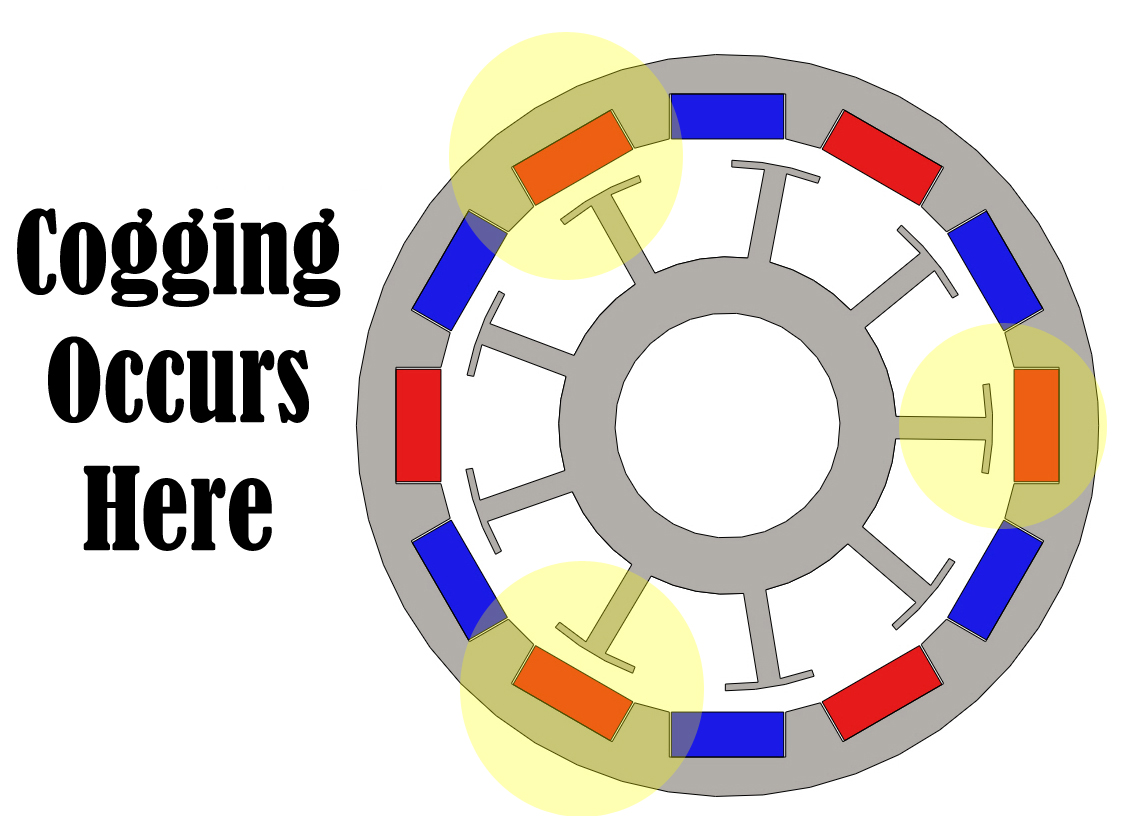
\includegraphics[width=0.4\linewidth]{Cogging.jpg}
\caption{\label{fig:cogging}}
\end{figure}

Cogging is the parasitic torque caused by the interaction between the metallic stator of a motor and the magnets from the rotor. Unfortunately, it is quiet high on our current motors, and create two issues : 
- It makes us feel small "bumps" and inconsistency in the movement and torque of the arm, due to these variations in torque depending on the position of the motor.
-High "deadband" for the motors and hence the arm : the cogging can be assimilated to a sort of high static magnetic friction, that prevent the motor from going to a precise position (high steady state error) when using a PD control loop. (Using integral control solve this issue, but also ruins the compliance of the arm).

\begin{figure}[H]
\centering
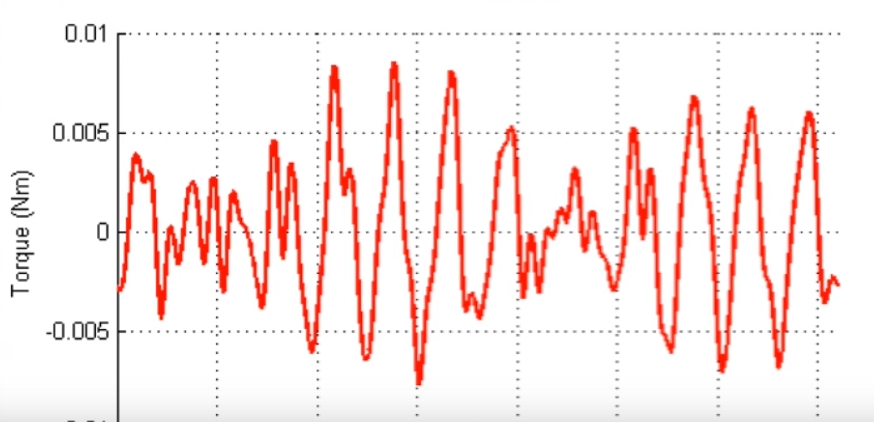
\includegraphics[width=0.4\linewidth]{anticogging.jpg}
\caption{\label{fig:anticogging}An example of the pattern of the cogging of a motor.}
\end{figure}

What I first did was to map the cogging using position control, and looking at the current used by the motor to hold a given position, I was able to get the cogging torque at this particular position. A Fourier analysis of the obtained data told me that our motor had two main frequency for cogging : 14Hz and 112Hz.
\vspace{0.1cm}
\\
This can be explained easily if we take a look at the geometry of a brushless motor. A brushless motor has slots, which are the branches of the stator, and poles pairs, which are the pairs of magnets on the rotor. Our motor has 24 slots and 14 pole pairs (28 magnets). The 14Hz is hence easy to understand, and 112Hz = 28*8Hz, Thus an harmonic of the geometry.
\vspace{0.1cm}
\\
Using the obtained datas, I set up a feed-forward in the control loop adding the opposite of the cogging into the control. Unfortunately, I was stupid at the time, thinking that the magnetic encoders were relative encoders, which was an issue for the start-up of the anticogging algorithm (because the cogging is dependant of the position of the motor obviously). These encoders are actually absolute encoder. So I tried to make the anticogging algorithm to start blindly at a local minimum, without really knowing where the motor was in the cogging pattern. This led to deceptive result.

\subsection{giving it another shot}

I wish I gave anticogging a better shot, several months later. Now that we know that the magnetic encoders are absolute, doing it should be quiet simpler. If someone want to try it again, the best ressources on it are \href{https://journals.sagepub.com/doi/full/10.1177/0278364915599045?casa_token=rXEpy4RR2b4AAAAA%3An0zk0MuxU2VKAQfZvDpCbwfNJZN7z-cub-tc2vSaLbtJPjbvZIVDb46b-iy0LtBiuBTFB1NyaS-JtA}{this paper} from Matthew Piccoli and Mark Yim, as well as the SimpleFOC discord, where there is a bunch of people that already tried to implement anticogging with different level of success.

\subsection{The future for motor drivers and motors}

If you decide on continuing using brushless motors, you can switch to \href{https://shop.odriverobotics.com/collections/motor-controllers/products/odrive-s1}{Odrives} motor drivers. Firstly, this way you won't need to switch the resistors each time. Secondly, the Odrives comes with a proprietary software (that you still can replace by SimpleFOC is you end up not wanting to use it). This software have an \href{https://docs.odriverobotics.com/v/latest/guides/anticogging.html}{anticogging algorithm} implemented, it could be interesting giving it a try before giving up on brushless motors.
\vspace{0.1cm}
Finally, we need to discuss about the motor. Switching to even larger outrunner brushless motor with less cogging and higher torque (low Kv number) (we will eventually need more torque if we want a bigger arm anyway). I personally would have loved to try the \href{https://www.aliexpress.us/item/3256807604192884.html?spm=a2g0o.productlist.main.17.110a7a10fF2ZxF&algo_pvid=a8f2c4a3-ed99-4828-aacc-8326e2a51cb4&algo_exp_id=a8f2c4a3-ed99-4828-aacc-8326e2a51cb4-8&pdp_ext_f=%7B%22order%22%3A%2220%22%2C%22eval%22%3A%221%22%7D&pdp_npi=4%40dis%21USD%2153.00%2153.00%21%21%2153.00%2153.00%21%40210390b817416169538974055ed688%2112000042212426335%21sea%21US%211753908079%21X&curPageLogUid=49xMA16m3Zkb&utparam-url=scene%3Asearch%7Cquery_from%3A}{Eaglepower LA8308} based on their online reputation in robotics.
\\
Otherwise, following Ken advice and switch to brushed motors may be the wisest choice, if the next person handling the project feels confident doing the switch to this type of motors.

\section{Conclusion}
To get a detailled conclusion on the learnings for each part of Testbed 2, read the end of each chapter, where there is different recommandation based on my experience with it. I don't know what is the next step for Testbed 2, apart for some control/sensing experiments to run on it. If you need any additional information/clarification on Testbed 2, you can reach me at \href{mailto:matthieu.prigent@student-cs.fr}{matthieu.prigent@student-cs.fr} .
\end{document}